\section{Markov Chain Monte-Carlo}
\label{chapter:MCMC}

\begin{markdown}
Dimensionality can be both a blessing and a curse. In \autoref{chapter:falikov_kimball_model} I'll discuss the fact that statistical physics can be somewhat boring in one dimension where most simple models have no phase transitions. This chapter is motivated by the the converse problem, high dimensional spaces can sometimes be just too much.

While there are many problems with high dimensions \footnote{my favourite being that there are no stable gravitational orbits in 4D and above} it's very hard to compute integrals over high dimensional spaces. If we take a discrete space with \(M\) dimensions each taking \(N\) distinct values. 
\end{markdown}




For a classical system, the thermal expectation value of some operator \(O\) is defined by a Boltzmann weighted sum over the classical state space:
\begin{align}
    \tex{O} &= \frac{1}{\Z} \sum_{\s \in S} O(x) P(x) \\
    P(x) &= \frac{1}{\Z} e^{-\beta F(x)} \\
    \Z &= \sum_{\s \in S} e^{-\beta F(x)}
\end{align}
While for a quantum system these sums are replaced by equivalent traces. The obvious approach to evaluate these sums numerically would be to directly loop over all the classical states in the system and perform the sum. But we all know know why this isn't feasible: the state space is too large! Indeed even if we could do it, it would still be computationally wasteful since at low temperatures the sums are dominated by low energy excitations about the ground states of the system. Even worse, in our case we must fully solve the fermionic system via exact diagonalisation for each classical state in the sum, a very expensive operation!~\footnote{The effort involved in exact diagonalisation scales like \(N^2\) for systems with a tri-diagonal matrix representation (open boundary conditions and nearest neighbour hopping) and like \(N^3\) for a generic matrix~\cite{bolchQueueingNetworksMarkov2006,usmaniInversionTridiagonalJacobi1994}.}

\clearpage
\begin{figure}
  \centering
  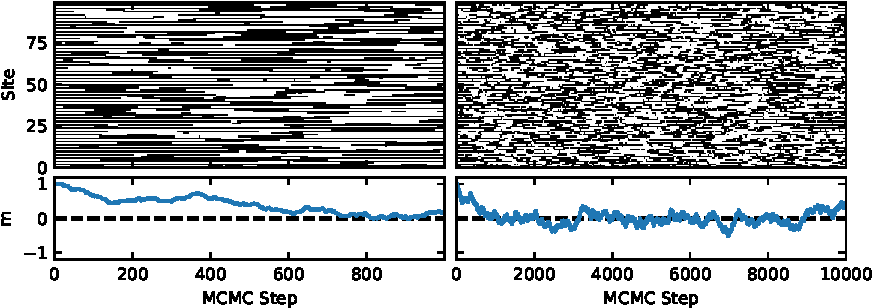
\includegraphics[width=\columnwidth]{figs/lsr/raw_steps_single_flip.pdf}
  \caption{An MCMC walk starting from the staggered charge density wave ground state for a system with \(N = 100\) sites and 10,000 MCMC steps. In this simulation only a single spin can be flipped per step according to the Metropolis-Hastings Algorithm. The staggered magnetisation \(m = N^{-1} \sum_i (-1)^i \; S_i\) order parameter is plotted below. At this temperature the thermal average of m is zero, while the initial state has m = 1. We see that it takes about 1000 steps for the system to converge, after which it moves about the m = 0 average with a finite auto-correlation time.  \(t = 1, \alpha = 1.25, T = 3, J = U = 5 \) \label{fig:raw}}
\end{figure}

\ac{MCMC} sidesteps these issues by defining a random walk that focuses on the states with the greatest Boltzmann weight. At low temperatures this means we need only visit a few low energy states to make good estimates while at high temperatures the weights become uniform so a small number of samples distributed across the state space suffice. However we will see that the method is not without difficulties of its own.

\begin{figure}
  \centering
  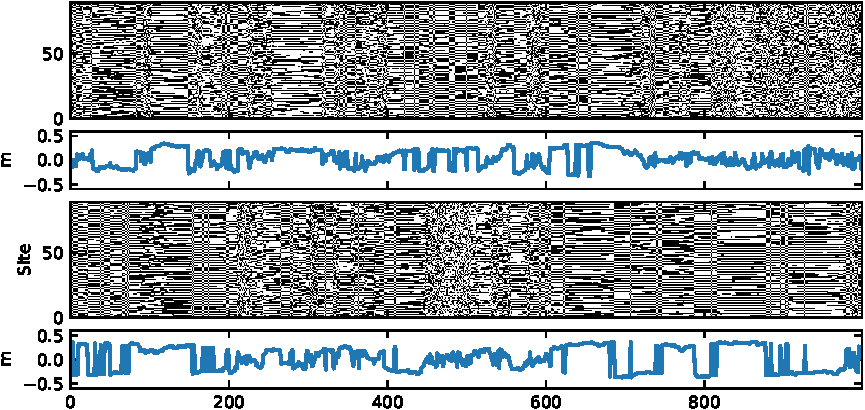
\includegraphics[width=\columnwidth]{figs/lsr/single.pdf}
  \caption{Two MCMC chains starting from the same initial state for a system with \(N = 90\) sites and 1000 MCMC steps.  In this simulation the MCMC step is defined differently: an attempt is made to flip n spins, where n is drawn from Uniform(1,N). This is repeated \(N^2/100\) times for each step. This trades off computation time for storage space, as it makes the samples less correlated, giving smaller statistical error for a given number of stored samples. These simulations therefore have the potential to necessitate \(N^2/100\) matrix diagonalisations for every MCMC sample, though this can be cut down with caching and other tricks. \(t = 1, \alpha = 1.25, T = 2.2, J = U = 5 \) \label{fig:single}}
\end{figure}

%MCMC from an ensemble point of view
In implementation \ac{MCMC} can be boiled down to choosing a transition function \(\T(\s_{t} \rightarrow \s_t+1) \) where \(\s\) are vectors representing classical spin configurations. We start in some initial state \(\s_0\) and then repeatedly jump to new states according to the probabilities given by \(\T\). This defines a set of random walks \(\{\s_0\ldots \s_i\ldots \s_N\}\). Fig.~\ref{fig:single} shows this in practice: we have a (rather small) ensemble of \(M = 2\) walkers starting at the same point in state space and then spreading outwards by flipping spins along the way. 

In pseudo-code one could write the MCMC simulation for a single walker as:

\begin{markdown}
```python
current_state = initial_state

for i in range(N_steps):
    new_state = sample_T(current_state) 
    states[i] = current_state
```
\end{markdown}

Where the \texttt{sample\_T} function here produces a state with probability determined by the \texttt{current\_state} and the transition function \(\T\).

If we ran many such walkers in parallel we could then approximate the distribution \(p_t(\s; \s_0)\) which tells us where the walkers are likely to be after they've evolved for \(t\) steps from an initial state \(\s_0\). We need to carefully choose \(\T\) such that after a large number of steps \(k\) (the convergence time) the probability \(p_t(\s;\s_0)\) approaches the thermal distribution \(P(\s; \beta) = \Z^{-1} e^{-\beta F(\s)}\). This turns out to be quite easy to achieve using the Metropolis-Hasting algorithm.

\subsection{Convergence Time}

Considering \(p(\s)\) as a vector \(\vec{p}\) whose jth entry is the probability of the jth state \(p_j = p(\s_j)\), and writing \(\T\) as the matrix with entries \(T_{ij} = \T(\s_j \rightarrow \s_i)\) we can write the update rule for the ensemble probability as:
\[\vec{p}_{t+1} = \T \vec{p}_t \implies \vec{p}_{t} = \T^t \vec{p}_0\]
where \(\vec{p}_0\) is vector which is one on the starting state and zero everywhere else. Since all states must transition to somewhere with probability one: \(\sum_i T_{ij} = 1\). 

Matrices that satisfy this are called stochastic matrices exactly because they model these kinds of Markov processes. It can be shown that they have real eigenvalues, and ordering them by magnitude, that \(\lambda_0 = 1\) and \(0 < \lambda_{i\neq0} < 1\). %https://en.wikipedia.org/wiki/Stochastic_matrix
Assuming \(\T\) has been chosen correctly, its single eigenvector with eigenvalue 1 will be the thermal distribution \footnote{or, in the general case, any desired distribution. MCMC has found a lot of use in sampling from the complicated distributions that arise when taking a Bayesian approach to statistics.} so repeated application of the transition function eventually leads there, while memory of the initial conditions decays exponentially with a convergence time \(k\) determined by \(\lambda_1\). In practice this means that one throws away the data from the beginning of the random walk in order reduce the dependence on the initial conditions and be close enough to the target distribution. 

\subsection{Auto-correlation Time}


\begin{figure}
  \centering
  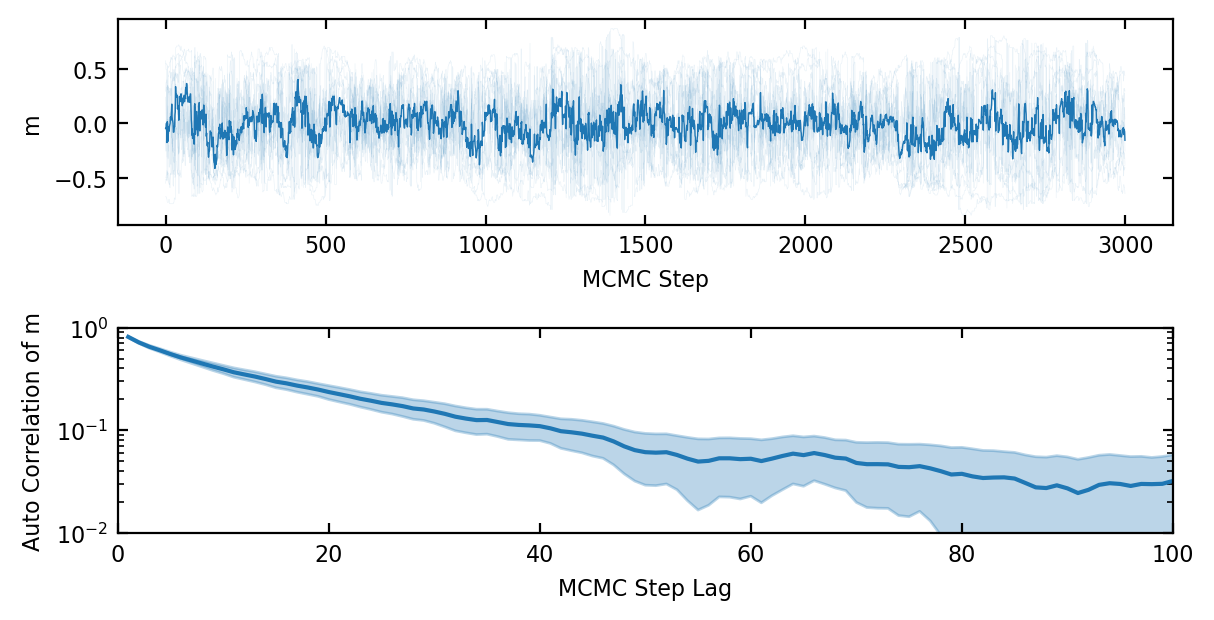
\includegraphics[width=\columnwidth]{figs/lsr/m_autocorr.png}
  \caption{(Upper) 10 MCMC chains starting from the same initial state for a system with \(N = 150\) sites and 3000 MCMC steps. At each MCMC step, n spins are flipped where n is drawn from Uniform(1,N) and this is repeated \(N^2/100\) times. The simulations therefore have the potential to necessitate \(10*N^2\) matrix diagonalisations for each 100 MCMC steps. (Lower) The normalised auto-correlation \((\expval{m_i m_{i-j}} - \expval{m_i}\expval{m_i}) / Var(m_i))\) averaged over \(i\). It can be seen that even with each MCMC step already being composed of many individual flip attempts, the auto-correlation is still non negligible and must be taken into account in the statistics. \(t = 1, \alpha = 1.25, T = 2.2, J = U = 5 \) \label{fig:m_autocorr}}
\end{figure}

At this stage one might think we're done. We can indeed draw independent samples from \(P(\s; \beta)\) by starting from some arbitrary initial state and doing \(k\) steps to arrive at a sample. However a key insight is that after the convergence time, every state generated  is a sample from \(P(\s; \beta)\)! They are not, however, independent samples. In Fig.~\ref{fig:raw} it is already clear that the samples of the order parameter m have some auto-correlation because only a few spins are flipped each step but even when the number of spins flipped per step is increased, Fig.~\ref{fig:m_autocorr} shows that it can be an important effect near the phase transition. Let's define the auto-correlation time \(\tau(O)\) informally as the number of MCMC samples of some observable O that are statistically equal to one independent sample.~\footnote{or equivalently as the number of MCMC steps after which the samples are correlated below some cutoff, see~\cite{krauthIntroductionMonteCarlo1996} for a more rigorous definition involving a sum over the auto-correlation function.} The auto-correlation time is generally shorter than the convergence time so it therefore makes sense from an efficiency standpoint to run a single walker for many MCMC steps rather than to run a huge ensemble for \(k\) steps each. 

Once the random walk has been carried out for many steps, the expectation values of \(O\) can be estimated from the MCMC samples \(\s_i\):
\[
    \tex{O} = \sum_{i = 0}^{N} O(\s_i) + \mathcal{O}(\frac{1}{\sqrt{N}})
\]
The the samples are correlated so the N of them effectively contains less information than \(N\) independent samples would, in fact roughly \(N/\tau\) effective samples. As a consequence the variance is larger than the \(\qex{O^2} - \qex{O}^2\) form it would have if the estimates were uncorrelated. There are many methods in the literature for estimating the true variance of \(\qex{O}\) and deciding how many steps are needed but my approach has been to run a small number of parallel chains, which are independent, in order to estimate the statistical error produced. This is a slightly less computationally efficient because it requires throwing away those \(k\) steps generated before convergence multiple times but it is a conceptually simple workaround.

In summary, to do efficient simulations we want to reduce both the convergence time and the auto-correlation time as much as possible. In order to explain how, we need to introduce the Metropolis-Hasting (MH) algorithm and how it gives an explicit form for the transition function. 

\subsection{The Metropolis-Hastings Algorithm}

MH breaks up the transition function into a proposal distribution \(q(\s \to \s')\) and an acceptance function \(\A(\s \to \s')\). \(q\) needs to be something that we can directly sample from, and in our case generally takes the form of flipping some number of spins in \(\s\), i.e if we're flipping a single random spin in the spin chain, \(q(\s \to \s')\) is the uniform distribution on states reachable by one spin flip from \(\s\). This also gives the nice symmetry property that \(q(\s \to \s') = q(\s' \to \s)\). 

The proposal \(\s'\) is then accepted or rejected with an acceptance probability \(\A(\s \to \s')\), if the proposal is rejected then \(\s_{i+1} = \s_{i}\). Hence:

\[\T(x\to x') = q(x\to x')\A(x \to x')\]

When the proposal distribution is symmetric as ours is, it cancels out in the expression for the acceptance function and the Metropolis-Hastings algorithm is simply the choice:
\[ \A(x \to x') = \min\left(1, e^{-\beta\;\Delta F}\right)\]
Where \(F\) is the overall free energy of the system, including both the quantum and classical sector.

To implement the acceptance function in practice we pick a random number in the unit interval and accept if it is less than \(e^{-\beta\;\Delta F}\):

\begin{lstlisting}[language=Python]
current_state = initial_state

for i in range(N_steps):
    new_state = proposal(current_state)
    df = free_energy_change(current_state, new_state, parameters)

    if uniform(0,1) < exp(-beta * df):
        current_state = new_state
        
    states[i] = current_state
\end{lstlisting}

This has the effect of always accepting proposed states that are lower in energy and sometimes accepting those that are higher in energy than the current state. 

\subsection{Choosing the proposal distribution}
\begin{figure}[H]
  \centering
  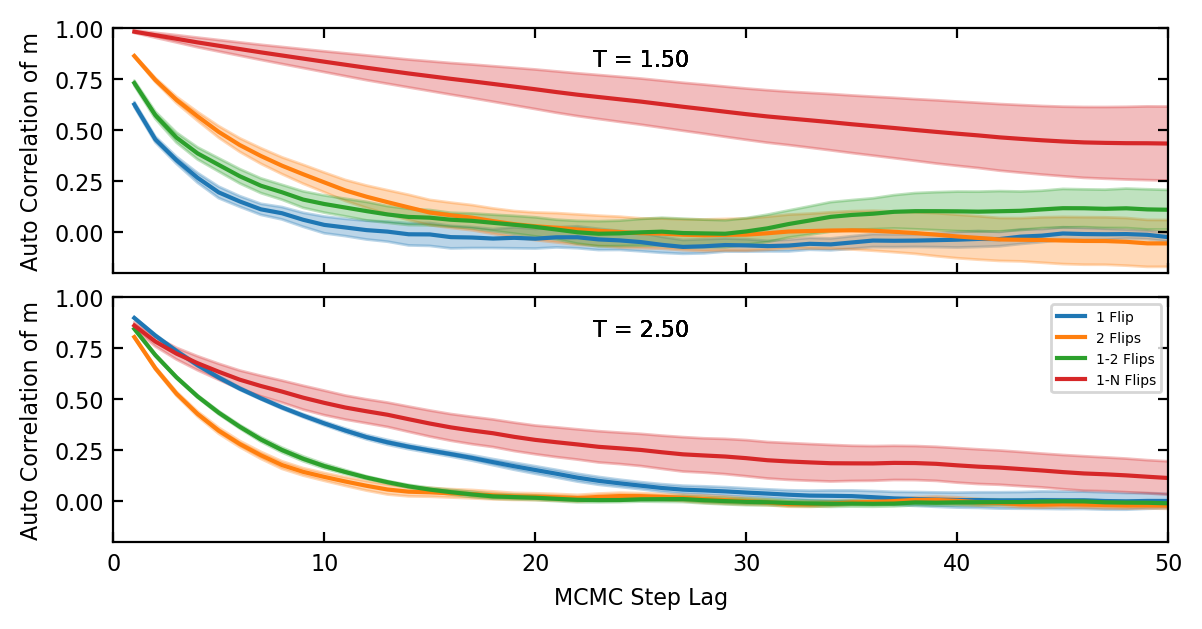
\includegraphics[width=\columnwidth]{figs/lsr/autocorr_multiple_proposals.png}
  Simulations showing how the autocorrelation of the order parameter depends on the proposal distribution used at different temperatures, we see that at \(T = 1.5 < T_c\) a single spin flip is likely the best choice, while at the high temperature \(T = 2.5 > T_c\) flipping two sites or a mixture of flipping two and 1 sites is likely a better choice. 
  \caption{ \(t = 1, \alpha = 1.25, J = U = 5 \) \label{fig:comparison}}
\end{figure}

Now we can discuss how to minimise the auto-correlations. The general principle is that one must balance the proposal distribution between two extremes. Choose overlay small steps, like flipping only a single spin and the acceptance rate will be high because \(\Delta F\) will usually be small, but each state will be very similar to the previous and the auto-correlations will be high too, making sampling inefficient. On the other hand, overlay large steps, like randomising a large portion of the spins each step, will result in very frequent rejections, especially at low temperatures. 

I evaluated a few different proposal distributions for use with the FK model. 

\begin{enumerate}
\item Flipping a single random site
\item Flipping N random sites for some N
\item Choosing n from Uniform(1, N) and then flipping n sites for some fixed N.
\item Attempting to tune the proposal distribution for each parameter regime.
\end{enumerate}

Fro Figure~\ref{fig:comparison} we see that even at moderately high temperatures \(T > T_c\) flipping one or two sites is the best choice. However for some simulations at very high temperature flipping more spins is warranted. Tuning the proposal distribution automatically seems like something that would not yield enough benefit for the additional complexity it would require.

\subsection{Two Step Trick}
Our method already relies heavily on the split between the classical and quantum sector to derive a sign problem free MCMC algorithm but it turns out that there is a further trick we can play with it. The free energy term is the sum of an easy to compute classical energy and a more expensive quantum free energy, we can split the acceptance function into two in such as way as to avoid having to compute the full exact diagonalisation some of the time:

\begin{lstlisting}[language=Python]

current_state = initial_state

for i in range(N_steps):
    new_state = proposal(current_state)

    df_classical = classical_free_energy_change(current_state, new_state, parameters)
    if exp(-beta * df_classical) < uniform(0,1):
        f_quantum = quantum_free_energy(current_state, new_state, parameters)
    
        if exp(- beta * df_quantum) < uniform(0,1):
          current_state = new_state
    
        states[i] = current_state
    
\end{lstlisting}
\FloatBarrier